\section{Methodology}
  \subsection{System Description}
    The system chosen for this work is taken from Chen's generalization in \cite{main}, but was originally proposed by Huang \& Li in \cite{huang1993theory}. In this paper, both approaches will be studied. The dynamic system was originally proposed as a first order differential equations system, but Chen's claims this can be generalized for fractional-order differential equation system. Thus, the systems are
    \begin{equation}
        \begin{array}{ll}
            \dot{X}&=Z+(Y-a)X\\
            \dot{Y}&=1-bY-X^2\\
            \dot{Z}&=-X-cZ\\
            &\textit{Original}
        \end{array}\qquad\Rightarrow\qquad
        \begin{array}{ll}
            \dfrac{d^{q_1}X}{dt^{q_1}}&=Z+(Y-a)X\\
            \dfrac{d^{q_2}Y}{dt^{q_2}}&=1-bY-X^2\\
            \dfrac{d^{q_3}Z}{dt^{q_3}}&=-X-cZ\\
            &\textit{Generalized}
        \end{array} \qquad q_1,q_2,q_3\in(0,1]
        \label{eq:main}
    \end{equation}
    This financial system describes the behavior of three state variables (i.e. $X$, $Y$, $Z$), which are respectively the interest rate, the investment demand and the price index; $a$, $b$ and $c$ are non-negative parameters that have real interpretation, these are (respectively): savings, cost per investment, elasticity of demand. We will give a short definition for each concept:
    \begin{itemize}
    \item Interest rate ($X$): is the cost of borrowed money, expressed as a percentage of the loan amount \cite{interestRate}.
    \item Investment demand($Y$): ``investment demand refers to the demand by businesses for physical capital goods and services used to maintain or expand its operations'' \cite{investmentDemand}.
    \item Price index ($Z$): measure of relative price changes \cite{priceIndex}.
    \item Savings ($a$): ``is what a person has left over when the cost of his or her consumer expenditure is subtracted from the amount of disposable income earned in a given period of time'' \cite{savings}.
    \item Cost per investment ($b$): also known as pre-operative cost, it is the necessary cost that we incurred in order to start an specific project.
    \item Elasticity of demand ($c$): ``measure of variable reaction to a change in another variable'' If  $c < 1$ is inelastic, in the other case is elastic \cite{elasticity}.
    \end{itemize}

	Previous studies claim that these equations (\ref{eq:main}) were obtained through analysis and a considerable number of experiments:
    \begin{itemize}
    \item $X$ comes from two important facts: first, the investment and savings are inversely proportional, and last the adjustment goods prices.
    \item $Y$ is in proportion with the rate of investment, and in proportion to inversion with the cost of investment and the the interest rate.
    \item The price index $Z$ depends on the inverse relationship between supply and demand of the commercial market; furthermore is related with the inflation rate. This is supposing that the amount of supplies and demands are constant\cite{jun2001study}. 
    \end{itemize}

	\subsection{Mathematical Model}
    
      Recall the dynamic system
      \begin{equation}
          \begin{array}{ll}
              \dfrac{d^{q_1}X}{dt^{q_1}}&=Z+(Y-a)X\\
              \dfrac{d^{q_2}Y}{dt^{q_2}}&=1-bY-X^2\\
              \dfrac{d^{q_3}Z}{dt^{q_3}}&=-X-cZ\\
          \end{array}
      \end{equation}
      For the original approach (i.e. integer order), will be treated as a specific case of the generalized model when  $q_1=q_2=q_3=1$. For the generalized model, since there are many definitions for fractional-order derivatives, the same definition as in Chen's paper will be used. Therefore, let us define the Caputo-type fractional derivative as 
      \begin{equation}
      	\dfrac{d^\alpha y}{dx^\alpha} = D_*^\alpha y(x) =  J^{m-\alpha}y^{(m)}(x), \quad \alpha > 0
      \end{equation}
      Where $m=\ceil{\alpha}$ is the ceil function of $\alpha$, $y^{(m)}$ is the $m$th ordinary derivative of $y$ and $J^{m-\alpha}$ is the Riemann-Liouville integral operator of order $m-\alpha$. This last operator is defined as
      \begin{equation}
      	J^\beta z(x) = \frac{1}{\Gamma (\beta)}\int_0^\infty{(x-t)^{\beta-1}z(t)dt}, \quad \beta > 0
      \end{equation}
      and $\Gamma(\beta)$ is the gamma function. For solving fractional differential equations, the Adams-Bashforth-Moulton predictor-corrector is used for numerical solutions; this method, introduced in \cite{diethelm2002predictor}, is presented in section \ref{sec:adam}.
      \subsection{Block Diagram}
      The following block diagram is only for the integer-order system with MathWork's Simulink, since the fractional order system was solved using Adams-Bashforth-Moulton predictor-corrector, in a standard Matlab script.
      
      \begin{figure}[H]
      	\centering
        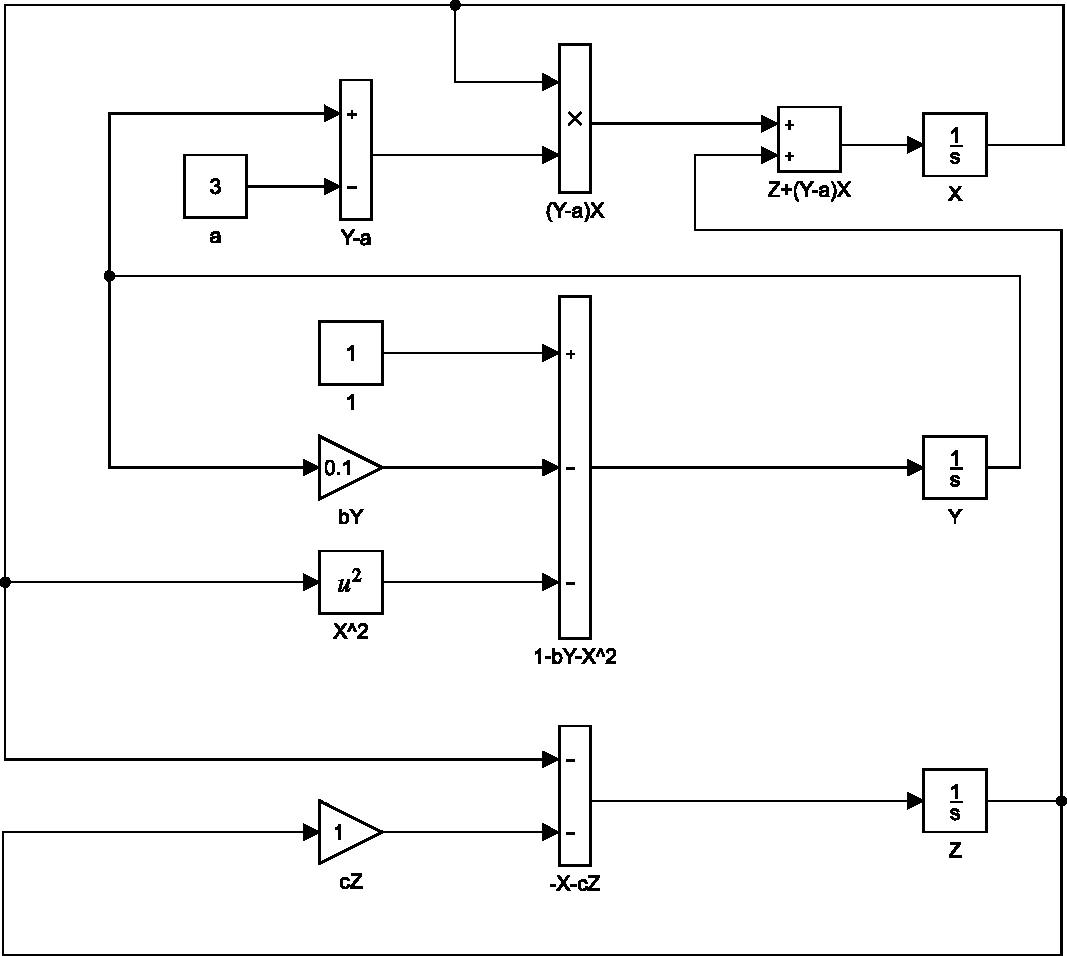
\includegraphics[scale=0.5]{files/DiagramaBloques.pdf}
        \caption{Block diagram for integer-order system.}
        \label{fig:block}
      \end{figure}
      
      \subsection{Simulation Method}
		\subsubsection{Adams-Bashforth-Moulton Algorithm}
        \label{sec:adam}
		Here the pseudo-code of the algorithm will be presented as in \cite{diethelm2002predictor}, this algorithm is applied to approximate the solution of a fractional differential equation 
        \begin{equation}
        	D_*^\alpha y(x) = f(x,y(x))
        \end{equation}
        
         where where $\alpha>0$ is the order of the differential equation, on a interval $[0,T]$.\\
        
        INPUT VARIABLES
        
        \begin{equation*}
        	\begin{array}{ll}
        		f &= \text{real-valued function defined for right side of the differential equation $D_*^\alpha y(x) = f(x,y(x))$}\\
                \alpha &= \text{the order of the fractional differential equation, real and positive number}\\
                y_0 &= \text{array of $\ceil{\alpha}$ initial conditions, i.e. $y(0),y'(0),...,y^{(\ceil{\alpha}-1)}(0)$}\\
                T &= \text{positive real-valued upper limit of the approximated solution interval}\\
                N &= \text{the number of steps that the method will take in the interval}\\ 
        	\end{array}
        \end{equation*}
        
        OUTPUT        
        \begin{equation*}
        	y = \text{an array of $N+1$ real numbers that contains the approximation for each value of $T/N$ in the interval}
        \end{equation*}
        
        %\pagebreak
        
        PROCEDURE
        \begin{lstlisting}
      h = T/N
      m = $\ceil{\alpha}$
      for $k=1$ to N do
      	$b[k]=k^\alpha-(k-1)^\alpha$
        $a[k]=(k+1)^{\alpha+1}-2k^{\alpha+1}+(k-1)^{\alpha+1}$
      end
      $y[0]=y_0[0]$
      for $j=1$ to N do
      	$P=\displaystyle\sum_{k=0}^{m-1}\limits\frac{(jh)^k}{k!}y_0[0]+\frac{h^\alpha}{\Gamma(\alpha+1)}\left[\displaystyle\sum_{k=0}^{j-1}\limits b[j-k]f(kh,y[k])\right]$
        $y[j]=\displaystyle\sum_{k=0}^{m-1}\limits\frac{(jh)^k}{k!}y_0[0]+\frac{h^\alpha}{\Gamma(\alpha+2)}\left[f(jh,P)+\left((j-1)^{\alpha+1}-f(0,y(0))(j-1-\alpha)j^\alpha\right)+\displaystyle\sum_{k=0}^{j-1}\limits a[j-k]f(kh,y[k])\right]$
      end
        \end{lstlisting}
        \subsubsection{Runge-Kutta Method}
        	Given the system to solve:
            \begin{equation}
            	y' = f(x,y)
            \end{equation}
            With the initial condition $y(0)=x_0$ and a specific time period to simulate the system $h$ the fourth order Runge-Kutta method dictates that the solution:
            \begin{equation}
            	y_{i+1} = y_i + \frac{h}{6}(k_1 + 2k_2 + 2k_3 + k_4)
            \end{equation}
            With:
            \begin{equation}
			\begin{array}{ll}
            	k_1 = f(x_i, y_i) \\
                k_2 = f(x_i + \frac{h}{2}, y_i + \frac{hk_1}{2}) \\
                k_3 = f(x_i + \frac{h}{2}, y_i + \frac{hk_2}{2}) \\
                k_4 = f(x_i + \frac{h}{2}, y_i + hk_3)
    		\end{array}
\end{equation}
		Furthermore, this method has different versions due to the application of different orders of this algorithm \cite{kutta}; therefore, it would be expected that this method is more precise than the Adam-Bashforth-Moulton because is three orders less compared to Runge-Kutta when both used to solve integer derivatives. On the other hand, there is no way to use the first method to solve fractional derivatives in higher orders (at least with reasonable complexities) therefore the Adam's algorithm has more computability than the Kutta's. 
            This method was used for the specific case for integer-order model i.e. $q_1=q_2=q_3=1$.
